\chapter{Tổng quan về Deep Learning}
\label{Chapter3}
\section{Mạng Nơ-ron nhân tạo}
Mạng nơ-ron nhân tạo là một mô hình lấy cảm hứng từ cấu trúc thần kinh của con người. Mỗi nơ-ron nhận tín hiệu đầu vào qua các liên kết của nó và chỉ tạo ra duy nhất một tín hiệu đầu ra. Tín hiệu đầu ra này được truyền theo các liên kết để đến các nơ-ron khác. Cứ như vậy, quá trình truyền và nội xử lý này được tiến hành cho đến nơ-ron cuối cùng để đưa ra một số quyết định tương tác với tín hiệu đầu vào. Từ cấu trúc trên, mô hình mạng nơ-ron nhân tạo được xây dựng như một hệ thống các nơ-ron và các kết nối giữa chúng. Tại mỗi điểm kết nối có hệ số liên kết nhằm giúp điều chỉnh tín hiệu đầu ra (như hình \ref{ANNStructures}). Quá trình học mạng nơ-ron chính là quá tình điều chỉnh các hệ số liên kết này sao cho phù hợp nhất với mục tiêu bài toán. Tại mỗi nơ-ron, tín hiệu vào sẽ được xử lý bằng một số phép biến đổi tuyến tính hoặc phi tuyến để tạo thành tín hiệu đầu ra. Thông thường, quá trình xử lý sẽ gồm 2 giai đoạn: giai đoạn tổng hợp tín hiệu đầu vào (thường bằng phép cộng tuyến tính) và giai đoạn biến đổi tín hiệu (thường bằng các hàm phi tuyến). \\


\begin{figure}[h]
	\centering
	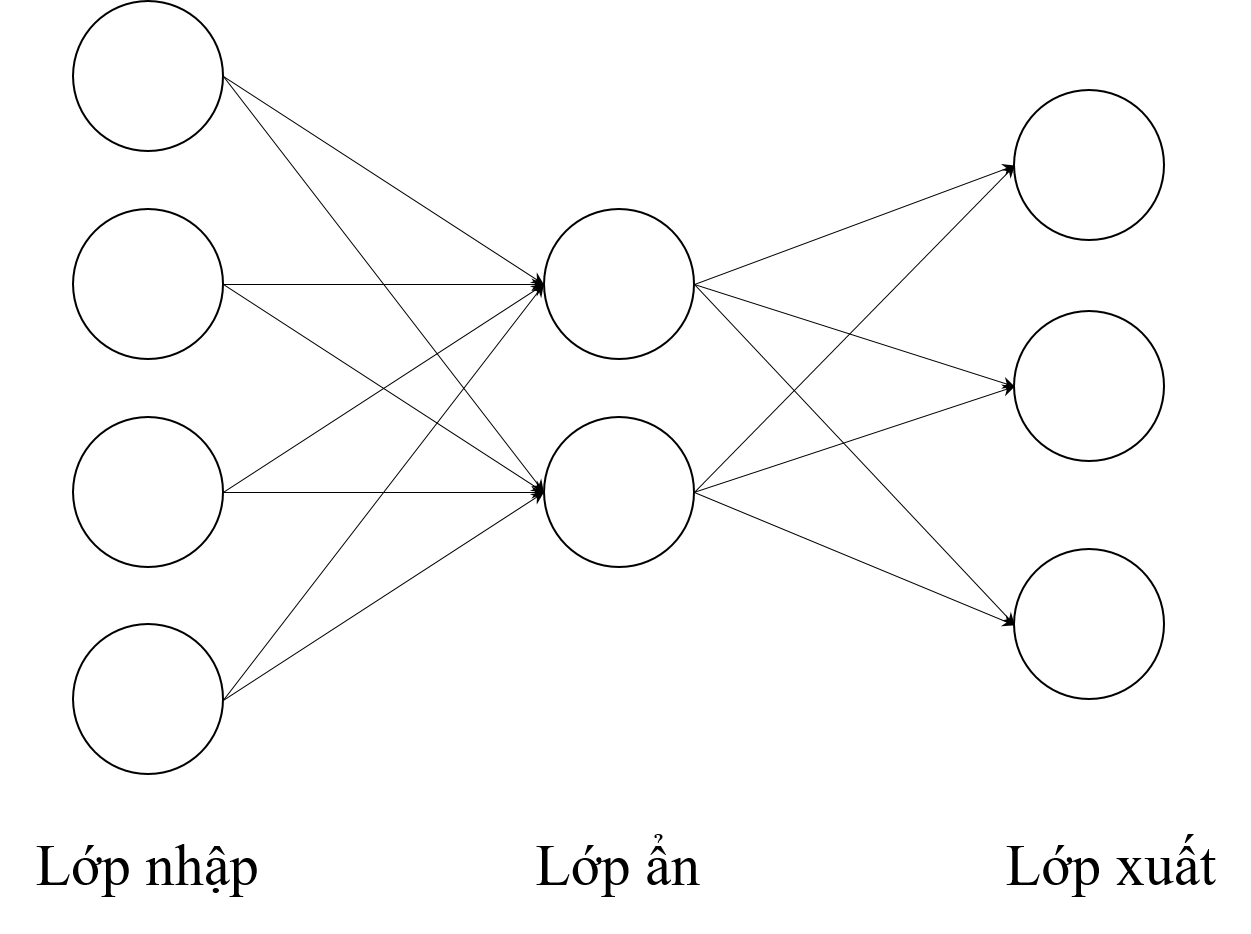
\includegraphics[width=0.68\textwidth]{Chapter3/ANNStructures}
	\caption{Cấu trúc mạng Nơ-ron nhân tạo}
	\label{ANNStructures}
\end{figure}


\section{Feed-forward Neural Network}

Feed-forward Neural Network (FFNN) là loại mạng đơn giản nhất trong các loại mạng Nơ-ron nhân tạo khác.  

\section{Recursive Neural Network}
\subsection{Recursive Neural Network}

\subsection{Recursive Auto-encoder Neural Network}


\section{Convolution Neural Network}


\section{Recurrent Neural Network}
\subsection{Recurrent Neural Network}
\subsection{Long Short Term Memory}




\section{Trích dẫn tài liệu}

Dùng lệnh  để trích dẫn một hoặc nhiều tài liệu tham khảo. Tài liệu tham khảo có thể là trang web~\cite{Listings,HDLVThS}, bài báo khoa học~\cite{1994-Cavnar}, sách~\cite{1984-TeX-Knuth,2006-DDien,2006-NPTV}, bài tạp chí~\cite{1989-TED} hoặc các nguồn tham khảo khác. 

Các tiểu mục của luận văn được trình bày và đánh số thành nhóm chữ số, nhiều nhất gồm bốn chữ số với số thứ nhất chỉ số chương (ví dụ: 4.1.2.1. chỉ tiểu mục 1 nhóm tiểu mục 2 mục 1 chương 4).
Tại mỗi nhóm tiểu mục phải có ít nhất hai tiểu mục, nghĩa là không thể có tiểu mục 2.1.1 mà không có tiểu mục 2.1.2 tiếp theo.

\section{Chèn mã nguồn}

Để chèn mã nguồn, cần dùng package listings~\cite{Listings}:

\begin{lstlisting}
\usepackage{listings}
\end{lstlisting}

Mã nguồn có thể được chèn trực tiếp như sau:

\begin{lstlisting}[language=Python]
print "Hello, World!"
\end{lstlisting}

hoặc chèn thông qua tập tin chứa mã nguồn trong thư mục ``SourceCode'' như sau:

\lstinputlisting[language=C++]{SourceCode/hello.cpp}

\section{Hình ảnh}

Để chèn hình ảnh, cần dùng package graphicx~\cite{Figures}:

\begin{lstlisting}
\usepackage{graphicx}
\end{lstlisting}

Hình \ref{fig:vd1}, hình \ref{fig:vd2} là một số ví dụ về chèn hình ảnh.

\begin{figure}[htp]
	\centering
	
\includegraphics[width=6 cm]{images/logo-khtn}
	\caption{Hình ví dụ 1}
	\label{fig:vd1}
\end{figure}

\begin{figure*}[htp]
	\centering
	
\includegraphics[width=40 mm]{images/logo-khtn}
	\caption{Hình ví dụ 2}
	\label{fig:vd2}
\end{figure*}

\section{Bảng biểu}

Để tạo bảng biểu, tham khảo thêm tại sharelatex.com~\cite{Tables}. Bảng \ref{tab:vd1} là một ví dụ về bảng.

\begin{table}[ht]
	\caption{Bảng ví dụ 1}
	\label{tab:vd1}%
	\begin{center}
		\begin{tabular}{ |p{3cm}||p{3cm}|p{3cm}|p{3cm}|  }
			\hline
			\multicolumn{4}{|c|}{Country List} \\
			\hline
			Country Name     or Area Name& ISO ALPHA 2 Code &ISO ALPHA 3 Code&ISO numeric Code\\
			\hline
			Afghanistan   & AF    &AFG&   004\\
			Aland Islands&   AX  & ALA   &248\\
			Albania &AL & ALB&  008\\
			Algeria    &DZ & DZA&  012\\
			American Samoa&   AS  & ASM&016\\
			Andorra& AD  & AND   &020\\
			Angola& AO  & AGO&024\\
			\hline
		\end{tabular}
	\end{center}
\end{table}

\section{Công thức}

Công thức có thể chèn vào trong cùng một dòng như $ \sqrt{a^2+b^2} $ hoặc nằm trên dòng riêng như sau:

\begin{equation}
x = a_0 + \frac{1}{a_1 + \frac{1}{a_2 + \frac{1}{a_3 + a_4}}}
\end{equation}
